\documentclass[11pt]{article}

\usepackage{latexsym}
\usepackage{amsmath}
\usepackage{amssymb}
\usepackage{amsthm}
\usepackage{graphicx}
\usepackage{wrapfig}
\usepackage{pseudocode}
\usepackage{url}
\usepackage{float}
\usepackage[backref, colorlinks=true, citecolor=red, urlcolor=blue, pdfauthor={Jyh-Ming Lien}]{hyperref}


\newcommand{\handout}[5]{
  \noindent
  \begin{center}
  \framebox{
    \vbox{
      \hbox to 5.78in { {\bf } \hfill #2 }
      \vspace{4mm}
      \hbox to 5.78in { {\Large \hfill #5  \hfill} }
      \vspace{2mm}
      \hbox to 5.78in { {\em #3 \hfill #4} }
    }
  }
  \end{center}
  \vspace*{4mm}
}

\newcommand{\lecture}[4]{\handout{#1}{#2}{#3}{#4}{#1}}

\newtheorem{theorem}{Theorem}
\newtheorem{corollary}[theorem]{Corollary}
\newtheorem{lemma}[theorem]{Lemma}
\newtheorem{observation}[theorem]{Observation}
\newtheorem{proposition}[theorem]{Proposition}
\newtheorem{definition}[theorem]{Definition}
\newtheorem{claim}[theorem]{Claim}
\newtheorem{fact}[theorem]{Fact}
\newtheorem{assumption}[theorem]{Assumption}

% 1-inch margins, from fullpage.sty by H.Partl, Version 2, Dec. 15, 1988.
\topmargin 0pt
\advance \topmargin by -\headheight
\advance \topmargin by -\headsep
\textheight 8.9in
\oddsidemargin 0pt
\evensidemargin \oddsidemargin
\marginparwidth 0.5in
\textwidth 6.5in

\parindent 0in
\parskip 1.5ex
%\renewcommand{\baselinestretch}{1.25}

\begin{document}

\lecture{Final Project Report: Automating Creation of Voting Districts}{Fall 2019}{William Austin}{CS 633 Computational Geometry}

\begin{abstract}
Gerrymandering poses a significant threat to the fairness of our elections by creating artificial advantages for one political party over another. The effect of this practice is easy to understand just by looking at the highly irregular districts produced, clearly engineered to include or exclude certain neighborhoods.  In recent years, there has been significant interest in improving the process of how these boundaries are drawn, and the movement to create districts that are compact and impartial is gaining bipartisan support. 

\medskip

Starting with information from the US census, we can use a data-driven approach that will employ algorithmic techniques to produce maps that are based solely on population distribution. This results in maps with that have favorable characteristicts and can be generated at a low cost and without political bias. The method that we focus on is based on `balanced centroidal power diagrams', which is related to the k-means clustering algorithm. We also identify a few metrics that can be used to quantitatively analyze the overall quality of districts so we can differentiate between one that is simple, compact, and contiguous, as opposed to one that is more complicated and likely to be gerrymandered. Our work is focused on maps for the state of Virginia, for both the state legislatures and the US House of Representatives.
\end{abstract}

\section{Motivation and Introduction}

In representative democracies, running fair elections that represent the will of the people is of critical importance. Gerrymandering undermines this effort by creating a set of maps that do not achieve this goal. However, as we will see, the practice is extremely common because the politicians that are in the current majority are usually also the ones that approve the maps. This leads to the common description of ``politicians picking their voters instead of voters picking their politicians". Therefore, this phenomenon is extremely hard to prevent, despite the fact that most people can identify a gerrymandered map with relative ease. As an example, the map below shows the current Virginia Congressional districts in northern Virginia. Congressional District 11 is good example of a non-compact district that has likely been modified for a political advantage.

\begin{figure}[H]
	\centering
	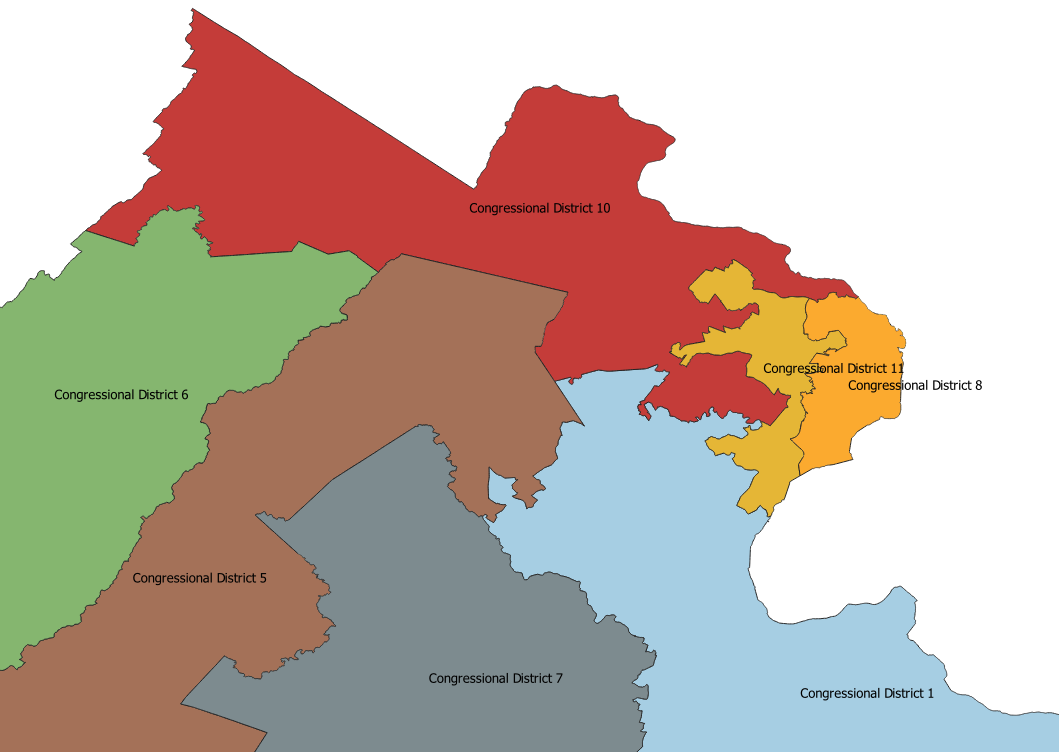
\includegraphics[width=0.55\textwidth]{GerrymanderingNOVA}
	\caption{Current Northern Virginia Congressional Districts}
	\label{fig:Gerrymandering_NOVA}
\end{figure}

Another example comes from southern Virginia, where the State Senate Districts 15 (brown) and 20 (green) look like a yin and yang symbol.

\begin{figure}[H]
	\centering
	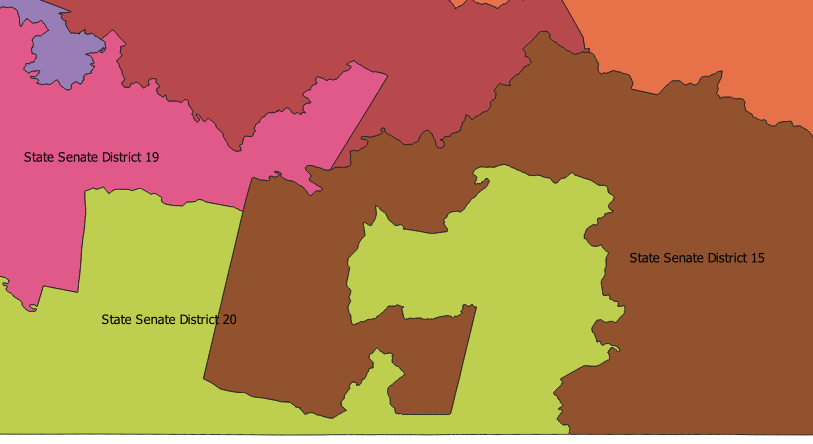
\includegraphics[width=0.55\textwidth]{Senate_15_20}
	\caption{Current Southern Virginia State Senate Districts}
	\label{fig:Gerrymandering_SOVA}
\end{figure}

\subsection{Brief History of Gerrymandering}

The term ``gerrymandering" comes from the an 1812 political cartoon in the Boston Gazette satirizing the map signed into law by then Governor Elbridge Gerry. The cartoon relates the shape of the districts to that of a salamander, which led people to refer to the map as the ``Gerry-mander". Subsequently, this phrase was shortened to gerrymander \cite{GerrymanderingWiki}.

\begin{figure}[H]
	\centering
	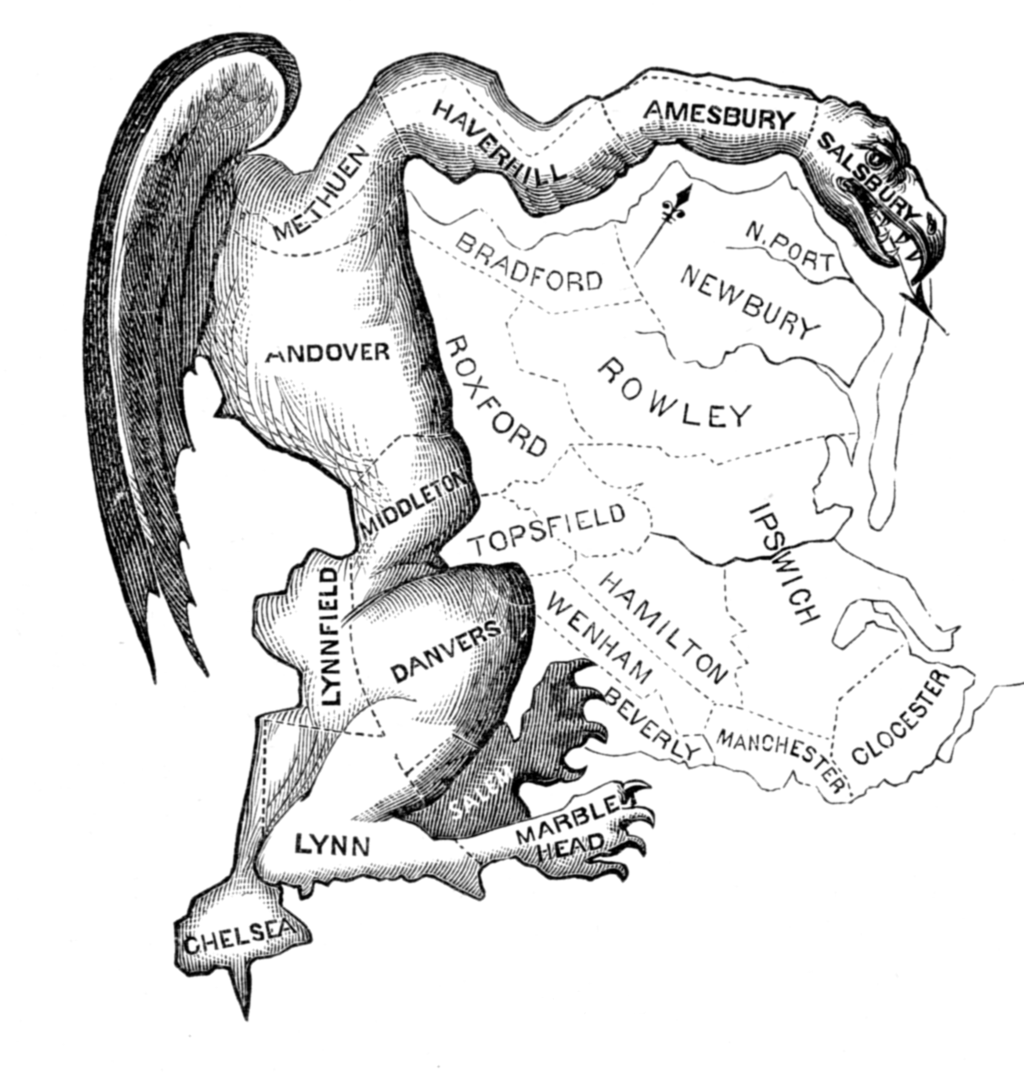
\includegraphics[width=.5\textwidth]{TheGerryMander}
	\caption{The Gerry-mander}
	\label{fig:The_Gerry_Mander}
\end{figure}

Since this original instance, gerrymandering has spread around the globe and there have been documented examples of the practice in more than 25 countries\cite{GerrymanderingWiki}.

\subsection{Recent Developments}

Clearly, the practice of gerrymandering has been around for a long time, but the last 20 years have seen it become much more common. In addition, as the effectiveness of these techniques have become evident, with REDMAP \cite{RedmapWiki}, we have seen efforts at a national party level to make gerrymandering a core component of the long term political strategy. This practice is sometimes referred to as ``cracking and packing" because a political organization wishes to organize districts so that opposing voters are split up, or ``cracked" among districts that they have an advantage in, or consolidated (``packed") into districts that they are likely to lose.

In addition to the effectiveness of previous applications, there are a few other factors that explain why this practice has become so common:
\begin{itemize}
	\item Running for public office and getting elected requires incredibly large amounts of money and effort. Maintaining a campaign staff, holding events, and purchasing advertisements are all required activities for winning an election, but not directly related to the role of a legislator. Therefore, there is an incredible incentive for government officials to rig the system to make re-election efforts easier.
	\item In most states (36 out of 50) \cite{GerrymanderingWiki}, the redistricting process is controlled by the state legislature, which is clearly going to be biased in favor of maps that keep the currently elected officials in office.
	\item More data is available than ever about how voters are distributed. By looking at poll results, historical data, and demographic trends, legislators can use gerrymandering systematically makes elections less competitive. This reduces the number of neighborhoods that will need to be targeted for a successful campaign, saving time and costs.
	\item Improved hardware makes analysis of all this data feasible in a reasonable amount of time. In addition, there are now more sophisticated software tools that can be used to determine how to most effectively alter district boundaries for political. In this paper, we explore ways of using algorithms and software to draw better districts, but deploying technology for political gain has been around much longer.
\end{itemize}

There are a few different strategies for dealing with this problem. Some states, including Virginia, are considering or have made structural changes that place the burden of drawing maps on an independent redistricting commission. The leading group supporting this type of reform is a bipartisan group called OneVirginia2021, with the long term goal of passing an amendment to the Virginia Constitution that maps describes how the redistricting process would work. An emphasis would be placed on process transparency, public involvement and removing the political influence of the state legislature \cite{OneVirginia2021Page}.

\medskip

Another national bipartisan group that is pushing for reform is FairVote. Their agenda includes gerrymandering reform as well as other structural changes in the voting process, such as Ranked Choice Voting. In 2011, FairVote sponsored a public competition to redraw the Virginia Congressional districts \cite{FairVotePage}.

\medskip

The most influential individual over the past decade in the area of programmatic creation of district boundaries is Brian Olson. He has created used data from the 2010 census to create new maps for almost every legislature in all 50 states. In addition, his site contains a collection of links to many other resources related to redistricting \cite{BrianOlsonRedistricting}. Olson is also very engaged trying to raise public awareness and is considered an expert in the field. His 2016 TED talk about the gerrymandering problem and his proposed solution has been viewed by thousands \cite{BrianOlsonTedTalk}. The image below shows his generated map for Virginia Congressional districts.

\begin{figure}[H]
	\centering
	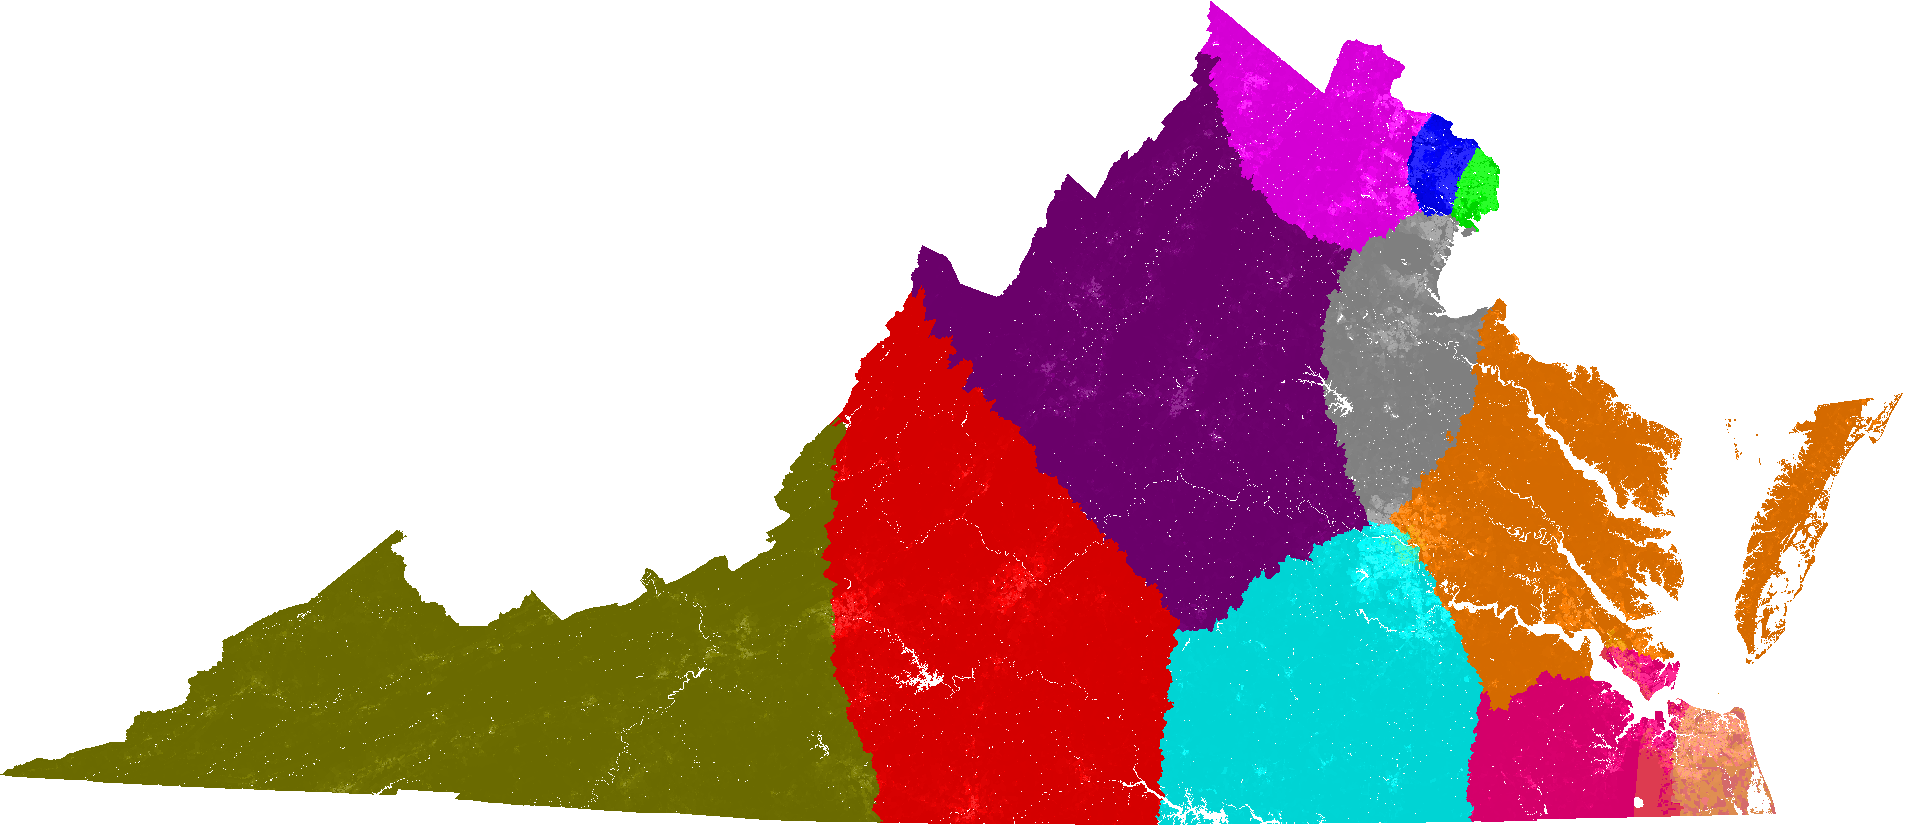
\includegraphics[width=\textwidth]{OlsonMap11}
	\caption{Proposed Virginia Senate Districts by Brian Olson}
	\label{fig:Olson_11_CD}
\end{figure}

\subsection{Overall Research Strategy}

The inspiration for this project was based on the 2018 paper, ``Balanced power diagrams for redistricting" \cite{cohenaddad2017balanced}. This paper provides the algorithmic basis for drawing maps with desirable properties that could represent legislative districts. More specifically, their criteria includes convexity, equal population distribution across regions, and shapes that have no more than six sides. Having these guaranteed properties is critical for producing fair and compact districts.   

\medskip

Because the original authors did not include sample maps for Virginia in their original paper, my primary goal was to generate these maps, using their methodology. However, I also wanted to enhance the work of the original authors by performing an additional postprocessing step that creates more useful maps that respect existing political boundaries, rather than the straight line Voronoi cells produced by their algorithm. Lastly, I wished to calculate some of the metrics proposed by Olson \cite{BrianOlsonMetrics} and others \cite{OtherMetrics}. Therefore, to summarize, the three main activities I performed were:
\begin{enumerate}
	\item Reproduce the work described in the paper by Cohen-Addad, Klein, and Young. Use the software available in their Bitbucket repository and run it on geospatial and demographic data collected for the state of Virginia. Generate maps for:
		\begin{itemize}
			\item Virginia Congressional Districts (11 districts)
			\item Virginia State Senate Districts (40 districts)
			\item Virginia House of Delegates Districts (100 districts)
		\end{itemize}
	\item Expand the set of maps produced in the first step to make them more useful by updating electoral district boundaries to respect census block divisions. 
	\item Investigate metrics for compactness and create scripts to perform calculations. These metrics should be calculated for both the old and new maps and compared. This establishes an argument for why this automated method of district creation may lead to better results than the traditionally hand-drawn districts. 
\end{enumerate}

\subsection{Technology and Software Tools Utilized}

Many different software products and technologies are required to perform the processing and analysis required for this project. Below, I give an overview of the main tools used, and what the function of each was.

\paragraph{Python 3.7.2}
Python is used extensively in the GIS (geographic information systems) domain and has excellent libraries that support common geospatial operations. In addition, Python is an extremely powerful general purpose scripting language, which makes it valuable for many other required tasks. In this project, the original authors used Python to format input and output, as well as to verify results and generate plotting data. Likewise, I used Python extensively to read and write shapefiles, aggregate data, compute metrics, and generate output files. Some of the critical Python libraries that I utilized were:
\begin{itemize}
	\item \textbf{PyShp 2.1.0}. This library makes it easy to read and write shapefiles, with support for operations like streaming and attribute retrieval.
	\item \textbf{Shapely 1.6.4} Shapely is a library that supports many geometric operations. For this project, we can create a Shapely polygon from the district definition and Shapely will perform operations such as centroid location, perimeter, area, and convex hull.
	\item \textbf{PyProj 2.4.2} This library allows us to read in data that is specified with a particular datum and CRS (coordinate reference system), and it will give us projected plane coordinates that we can use to perform geometric operations on.
\end{itemize}

\paragraph{C++ 11} The algorithm provided by the paper's author has been implemented in C++. This code allows us to compute the desired balanced centroidal power diagram. I was able to clone their repository and run a successful build to create the desired executable, but a few minor changes to their original source code were required.

\paragraph{QGIS 3.10.0} QGIS is a general purpose tool for viewing, analyzing, and editing geospatial data. In this project, the main purpose was for modifying shapefiles. Some of the key operations supported are:
\begin{itemize}
	\item Geospatial joins, which allow us to merge data from different maps together, based on a common key attribute. In this project, we added the census block population data from a spreadsheet to the shapefile as an attribute by using this feature.
	\item Centroid calculations, which allow us to compute the centroid of a district or census block. This is useful because the balanced centroidal power diagram algorithm requires single points as input, so we represent census blocks by their centroid. In addition, the average distance metrics depend on knowing what the district centroid is.
	\item Unions and intersection operations. We can use these capabilities to transform the Voronoi cells in the algorithm output into a valid shapefile by retrieving the intersection with the Virginia state shapefile and the removing unwanted features. In addition, we can merge census blocks into a single region to produce our final modified output.
	\item Styling maps with colors, labels, and transparency to generate images for our output.
\end{itemize}

\paragraph{Gnuplot 5.2} This tool was used by the original authors to generate visual output for the generated maps.


\subsection{Project Artifacts}
All code and project aritifacts are avaiable on my public GitHub account. The URL is:

\begin{center}
	\url{https://github.com/william-r-austin/district2}
\end{center}

\section{Methods Used and Studied}
In this section, we will describe the algorithms and processes needed to produce our output. In addition, we give the mathematical basis for our metrics. 

\subsection{Balanced Centroidal Power Diagrams}
This algorithm is the basis for our work. As described by the authors of the original paper \cite{cohenaddad2017balanced}, this is an iterative algorithm that repeatedly assigns population points  to districts based on a weighted distance, and then updates the center of the district according to these assignments. This algorithm, like other ones similar to it, must balance the shape of the produced districts and how compact they are with the how evenly the population is distributed. In this case, the authors use a balanced power diagram, which guarantees equal population distribution, and by requiring district centers to coincide with district centroids, they produce Voronoi cell shaped districts, which must be compact. The high-level logic pseudocode for the method is given here.

\begin{figure}[H]
	\centering
	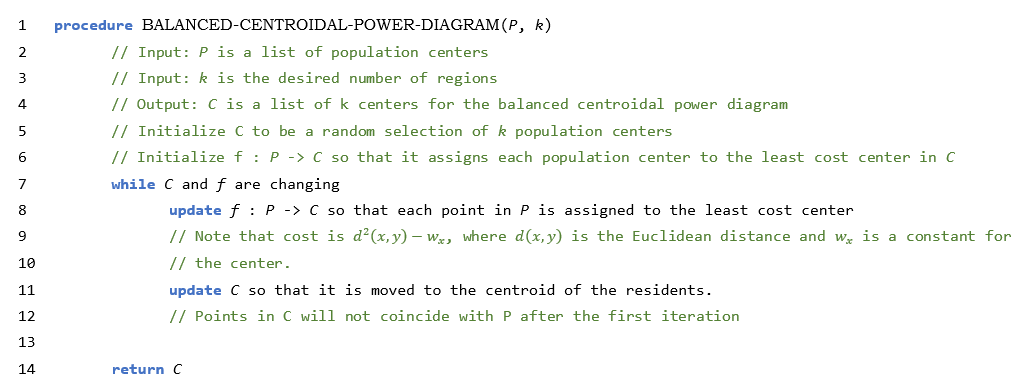
\includegraphics[width=\textwidth]{pseudocode}
	\caption{Pseudocode for Computing Balanced Centroidal Power Diagrams}
	\label{fig:BCPD}
\end{figure}

Note that this problem can be transformed to a version of the transshipment problem which can be solved using minimum-cost flow algorithms \cite{TransshipmentWiki}. This makes the solution much more efficient a practical than a brute force approach.

\medskip

In the authors code, the main logic for iteratively choosing the centers is implemented in $redistrict.cpp$. The mincostflow.cpp class is a minimum cost flow solver that was included to efficiently compute the assignments to each district center. The image below shows an example of running the application and this particular example takes about 4 seconds to run. In addition to the console output, a file is produced that contains the exact district centers, as well as the district assignments for all of the input points. 

\begin{figure}[H]
	\centering
	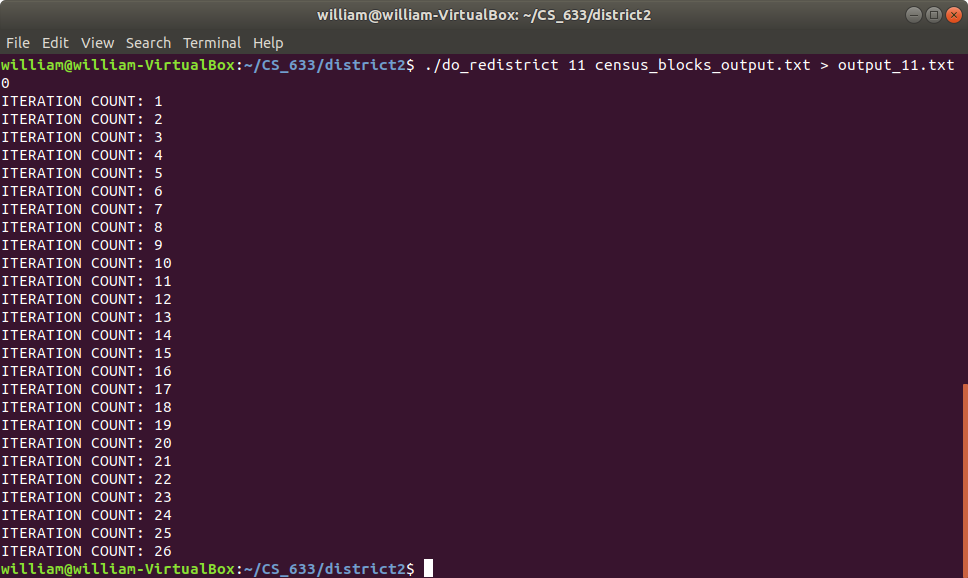
\includegraphics[width=.55\textwidth]{do_redistrict}
	\caption{Sample Execution of the \texttt{do\_redistrict} Application with k = 11}
	\label{fig:doredistrict}
\end{figure}


\subsection{Methodology for Map Creation}

Now, we will give an overview of the all the steps needed to generate a map based on population data. This process must integrate data from many different sources and we will explain in more detail how the different tools that we mentioned earlier are used.

\paragraph{Step 1. Data Collection for Virginia}

The first step for creating maps is to collect the required geospatial information and population data for the state. The most commonly used file type for representing a this information is the shapefile (SHP) format, and there are many different sources that we can use to obtain these and not all of them give us the information that we need. Below is a list of the data sources used for this project.
\begin{itemize}
	\item The final census block data and VA State Senate district shapefiles came from the Census bureau website \cite{TigerBG} \cite{VA_SLDU}. These shapefiles distributed by the Census bureau are called TIGER files because they are stored in the Topoligically Integrated Geographic Encoding and Referencing database.
	\item The population data came from the American Fact Finder website \cite{AFF}. Understanding the layout of the data sources and creating a query to return the data that we were looking for took some time. Understanding the hierarchy of geographic entities and how they are related is critical to being able to efficiently retrieve data. Many of the conventions rely on the listof LSAD (legal/statistical area description) codes. However there are plenty of resources available on the Census site that describe these relationships\cite{CensusGeoHelp}. The final  search criteria and resulting CSV file are shown below. 
	\begin{figure}[H]
		\centering
		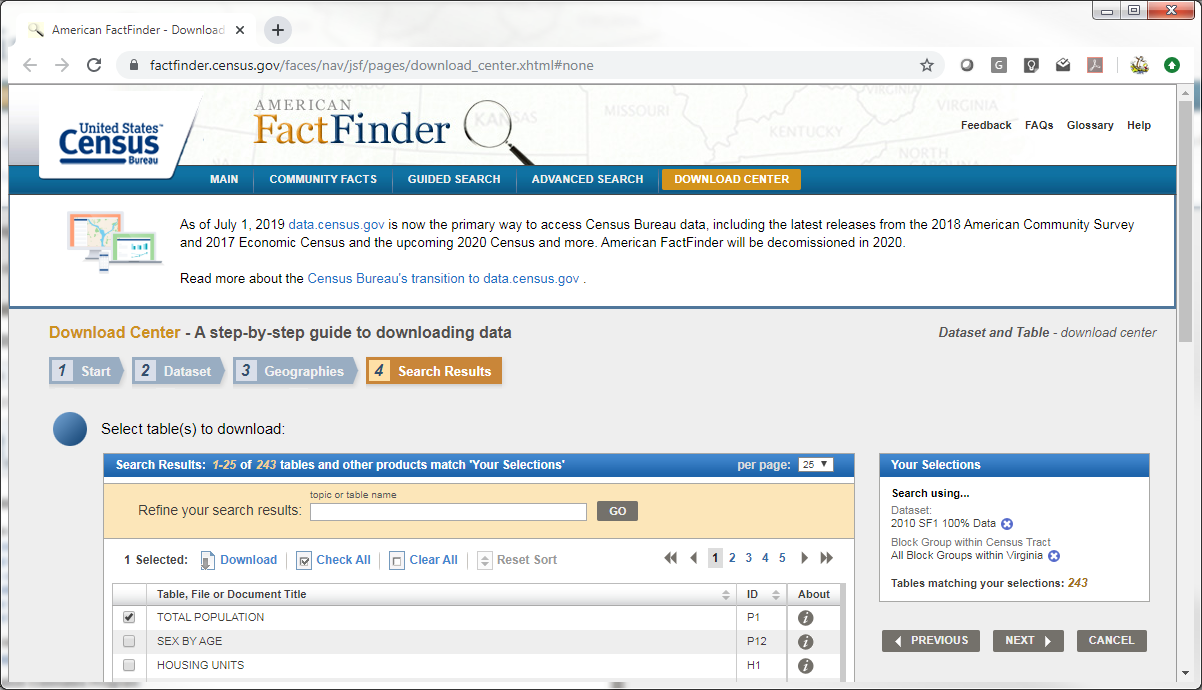
\includegraphics[width=.6\textwidth]{aff}
		\caption{American Fact Finder Population by Block Group Search}
		\label{fig:dewnfiweofn}
	\end{figure}
	\begin{figure}[H]
		\centering
		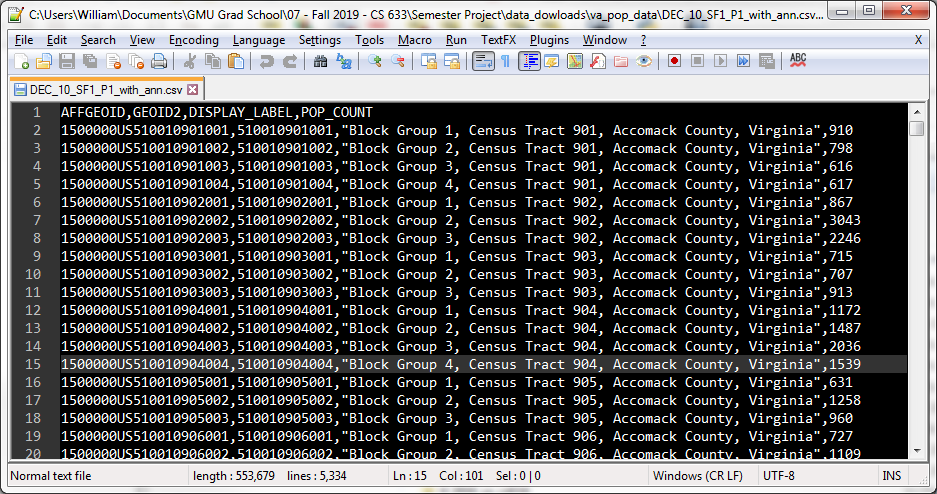
\includegraphics[width=.6\textwidth]{popdata}
		\caption{Format of Downloaded 2010 Census Population Data}
		\label{fig:dewnfnfwieof}
	\end{figure}
	\item The Virginia Congressional Districts also came from the \url{data.gov} website, which is also run by the Census bureau \cite{VA_CD_116}.
	\item Lastly, the shapefile for the Virginia House of Delegates came from the Virginia Roads website, which is run by the Virginia Department of Transportation (VDOT) \cite{VA_Roads}. An example of what the raw shapefile looks like in QGIS is shown here. The other raw shapefiles are similar.
	\begin{figure}[H]
		\centering
		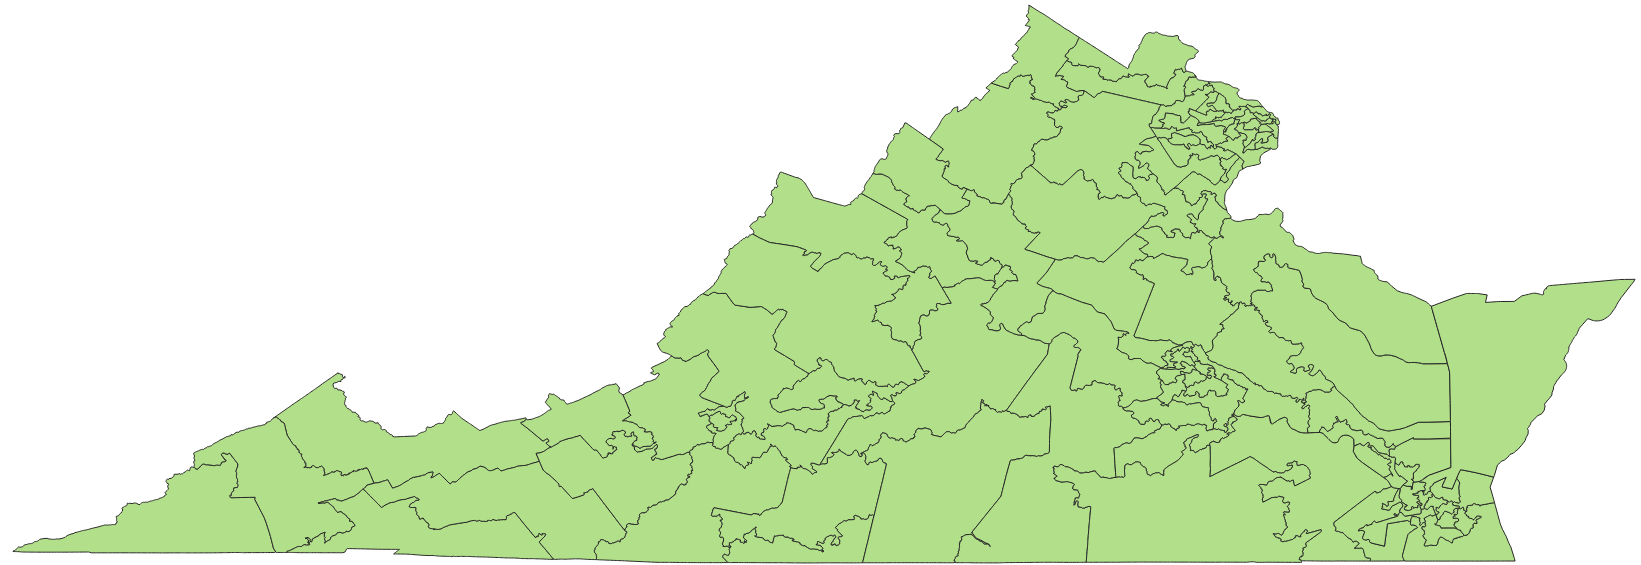
\includegraphics[width=.6\textwidth]{DelegatesRaw}
		\caption{Raw Virginia House of Delegates Shapefile}
		\label{fig:delegatesraw}
	\end{figure}
\end{itemize}

\paragraph{Step 2. Format Population and Census Block Data for Algorithm}
In order to compute the balanced centroidal power diagram, we must provide a set of points and their associated weights. In our case, these points will be the latitude and longitude for the centroids of the 5301 census blocks in Virginia, and the weight will simply be the population for that census block.

\medskip

To create this required input file, we start by calculating the centroids for each block in QGIS and adding the latitude and longitude of this point as the \texttt{XCOORD} and \texttt{YCOORD} feature attributes. The calculated centroids are shown below.
\begin{figure}[H]
	\centering
	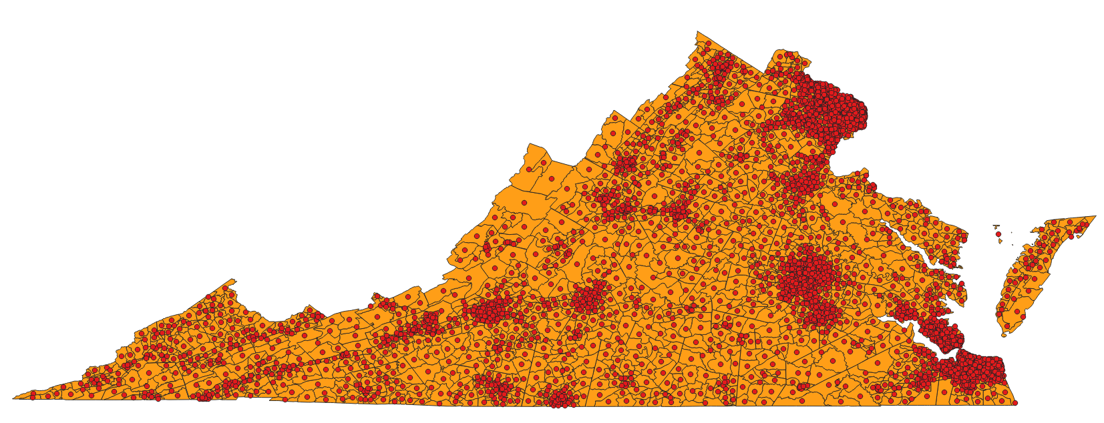
\includegraphics[width=.55\textwidth]{CensusBlockCentroids}
	\caption{Calculated Centroids for each Census Block}
	\label{fig:doredistricrewrwet}
\end{figure}

Next, we use the ``geospatial join" feature of QGIS to merge the population data from the downloaded CSV into the shapefile. We join on the \texttt{AFFGEOID} (American Fact Finder Geographic Identifier), which is present in both data sets. The population for each census block is save as the \texttt{POPCOUNT} attribute for each feature.

\medskip

Lastly, we created a Python scrip named $combine\_data.py$ that reads the combined shapefile and writes a text file in the desired format. As expected, this script makes use of the PyShp library to read the desired attributes from the saved shapefile. The first few lines of this file are shown below.

\begin{figure}[H]
	\centering
	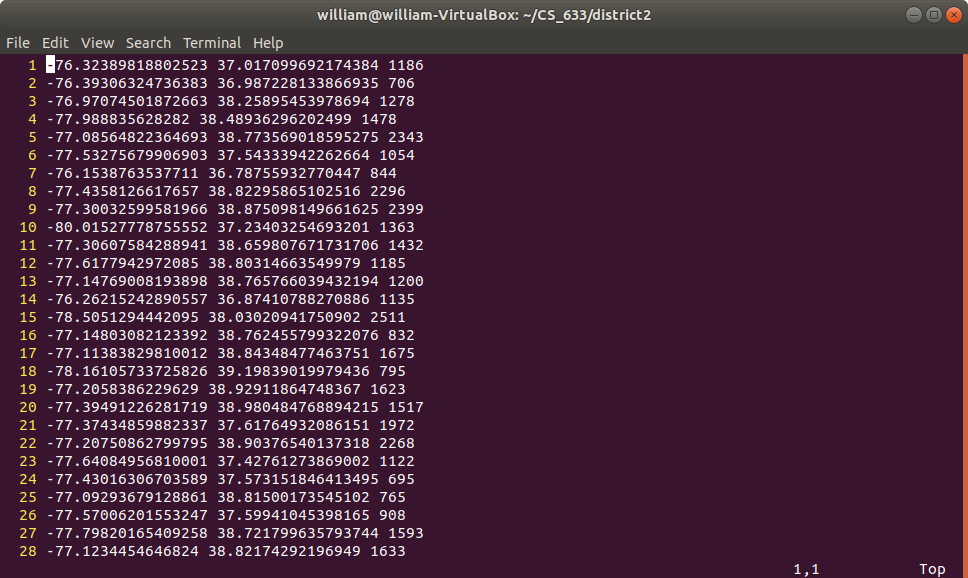
\includegraphics[width=.55\textwidth]{cbfile}
	\caption{Census Block Centroids and Population Counts}
	\label{fig:cbfsturfff}
\end{figure}

\paragraph{Step 3. Run Application to Create Maps for Virginia}

Earlier, while describing the balanced centroidal power diagrams algorithm, we showed the sample output from the application. See \ref{fig:doredistrict} for details. At this step, we decide $k$, which represents the number of districts, and the application will assign each population point to one of these districts. Sample output from for $k$ = 11 is shown below.

\begin{figure}[H]
	\centering
	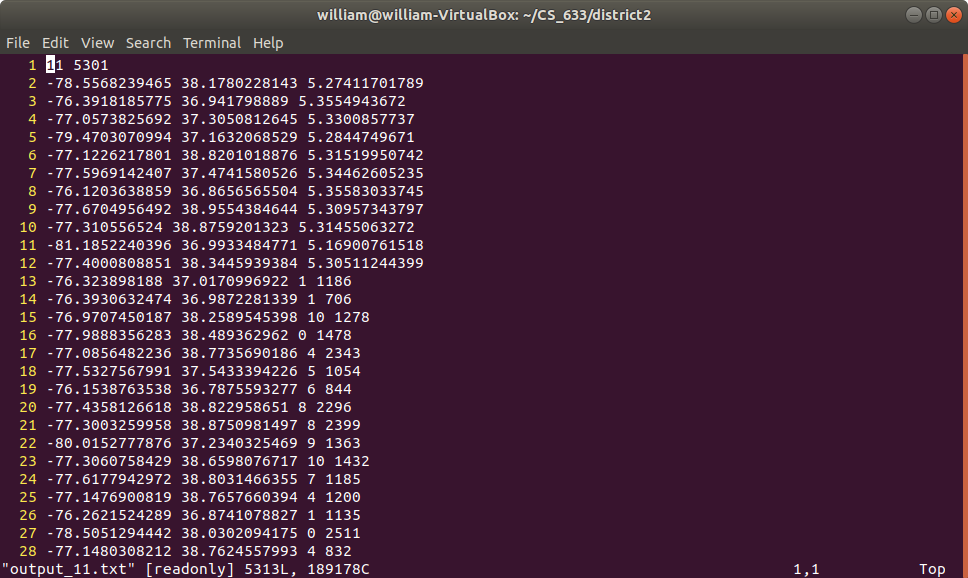
\includegraphics[width=.55\textwidth]{appoutput}
	\caption{Sample Output from Balanced Centroidal Power Diagram Algorithm}
	\label{fig:outputzzz}
\end{figure}

The last part of this step is to use Python to format the algorithm output correctly for gnuplot. There are two steps that need to be completed to show the map properly:
\begin{enumerate}
	\item The $Voronoi\_boundaries.py$ script generates the correct edges for the resulting diagram and associates each generated district and all population points within that district to a particular color.
	\item The $plotGNUPlot.py$ script will generate the gnuplot output and uses an additional boundary file to clip the Voronoi cells to match the geography of the state.
\end{enumerate}

\begin{figure}[H]
	\centering
	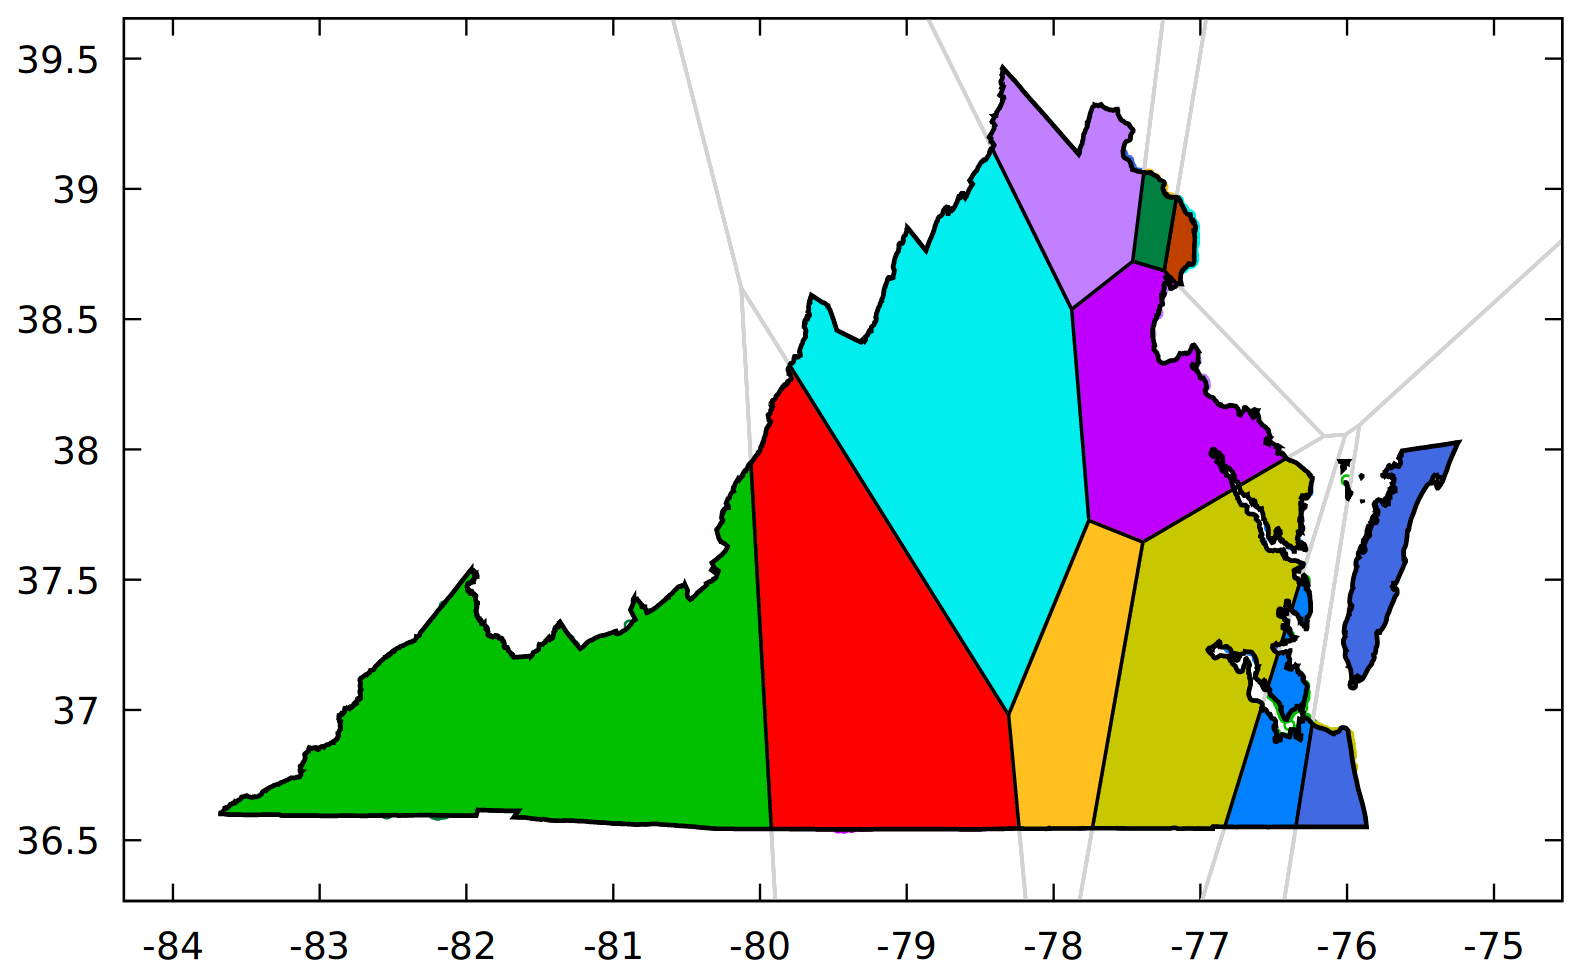
\includegraphics[width=.55\textwidth]{VoronoiMap11}
	\caption{Balanced Centroidal Power Diagram Map for 11 Congressional Districts, using GNUPlot}
	\label{fig:vmap11}
\end{figure}

\paragraph{Step 4. Use Map Output to Create Standard Shapefiles}

This step is a necessary conversion procedure to generate a shapefile that matches the generated map from the previous step. There are several steps involved in this step, descibed below:

\begin{enumerate}
	\item Extract the raw Voronoi cells from the output file generated in the previous step.
	\item Create and run a Python script that generates a shapefile from the extracted data. In my code, this is the $CreateShapefile.py$ script. This script will create a shapefile with the correct regions.
	\item Open the generated shapefile with our Voronoi cells, as well as a shapefile with the Virginia state outline in QGIS. The image below shows what this looks like.
	\begin{figure}[H]
		\centering
		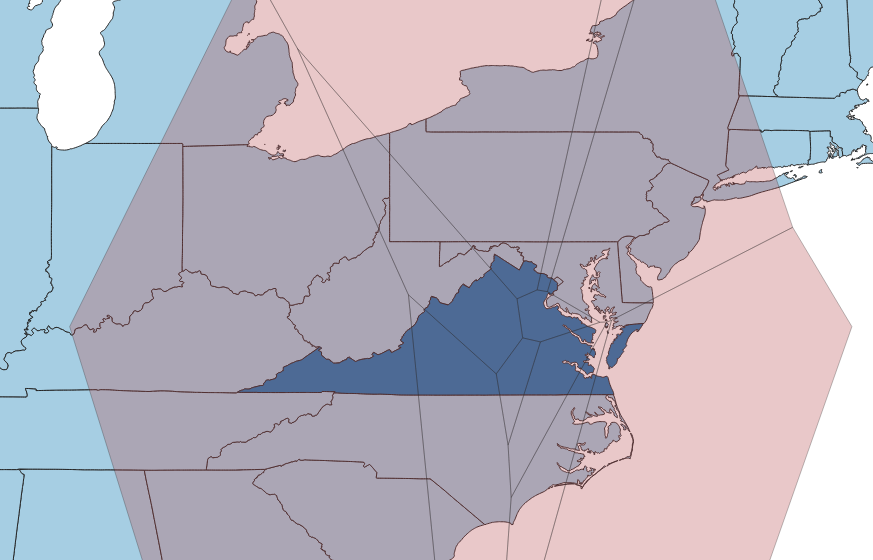
\includegraphics[width=.6\textwidth]{5a3_Overlay}
		\caption{Voronoi Cell Shapefile Overlaid on US State map}
		\label{fig:vcusmap}
	\end{figure}
	\item Use the QGIS functions to intersect these layers and generate a new layer. Remove all extraneous features, give each district a proper name, apply a reasonable style, and save the resulting shapefile. The result is below.
	\begin{figure}[H]
		\centering
		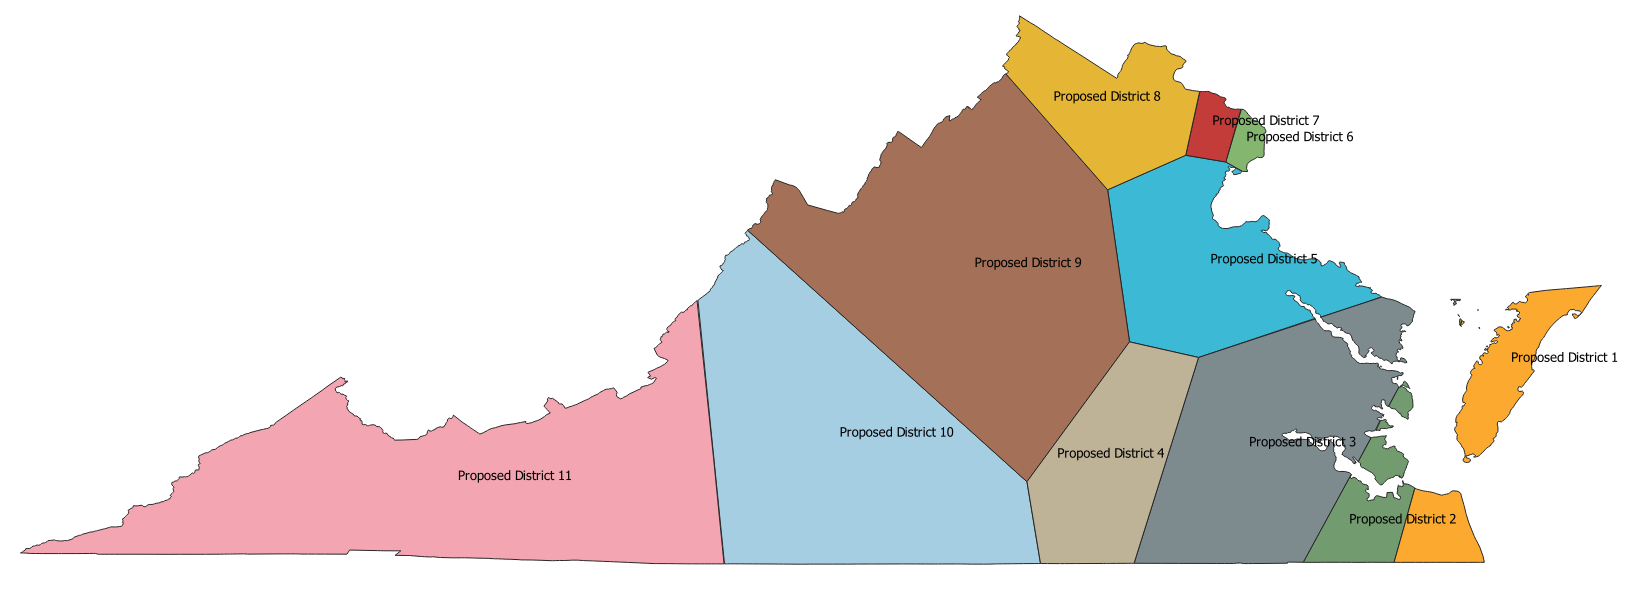
\includegraphics[width=.6\textwidth]{5a4_Final}
		\caption{Shapefile Representing Balanced Centroidal Power Diagram Output}
		\label{fig:shp4bcpd}
	\end{figure}
\end{enumerate}

\paragraph{Step 5. Generate District Maps Without Splitting Census Blocks}

The enhancement that we implemented on top of this output is to create a map that is slightly modified, but respects census block boundaries. The main work for this step is to create a Python script that reads all of the census block and compares them to the generated Voronoi cells for our existing map. Then, we assign each census block to the district that it has the most area overlap with. One interesting optimization is that we can easily compute a bounding box around each census block and Voronoi cell so that we can save quite a bit of processing time by simply not comparing regions that do not overlap. This functionality is implemented in $EvaluateCensusBlocks.py$. 

\medskip

Note that the the output of this script is a CSV file that contains the mapping of \texttt{AFFGEOID} identifiers for each census block, along with the assigned district number. Then, we can perform a geospatial join to integrate this data into our census block shapefile. The CSV file data is shown below.

\begin{figure}[H]
	\centering
	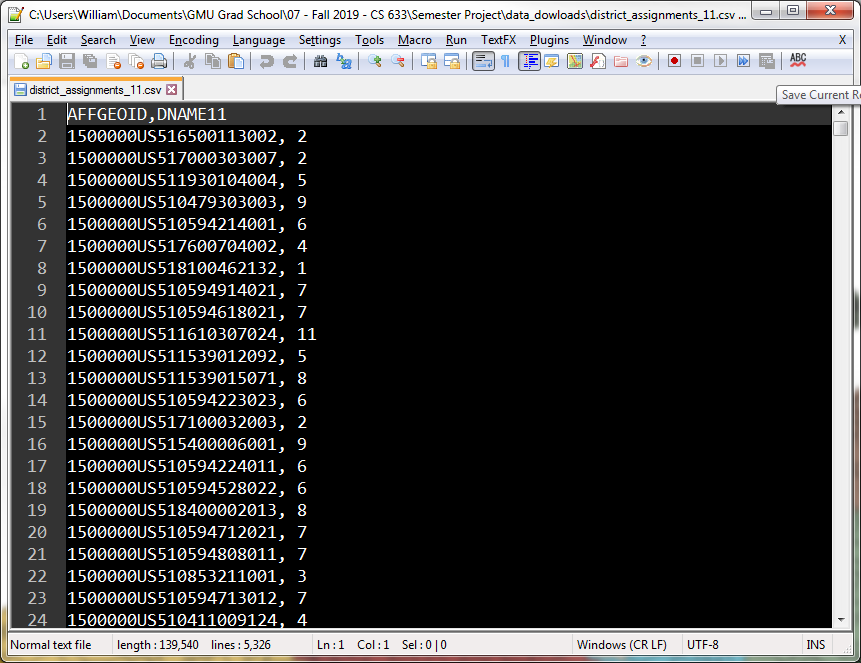
\includegraphics[width=.55\textwidth]{da11}
	\caption{Python Script Output, with Census Block Assignments}
	\label{fig:cbass11}
\end{figure}

\medskip

The last step for creating the final map is to use the QGIS ``Dissolve" function to create a single region from many individual regions. In this case, all features that have the same district mapping can be dissovled into a single feature. This generated layer can then be exported as a new shapefile, as shown below.

\begin{figure}[H]
	\centering
	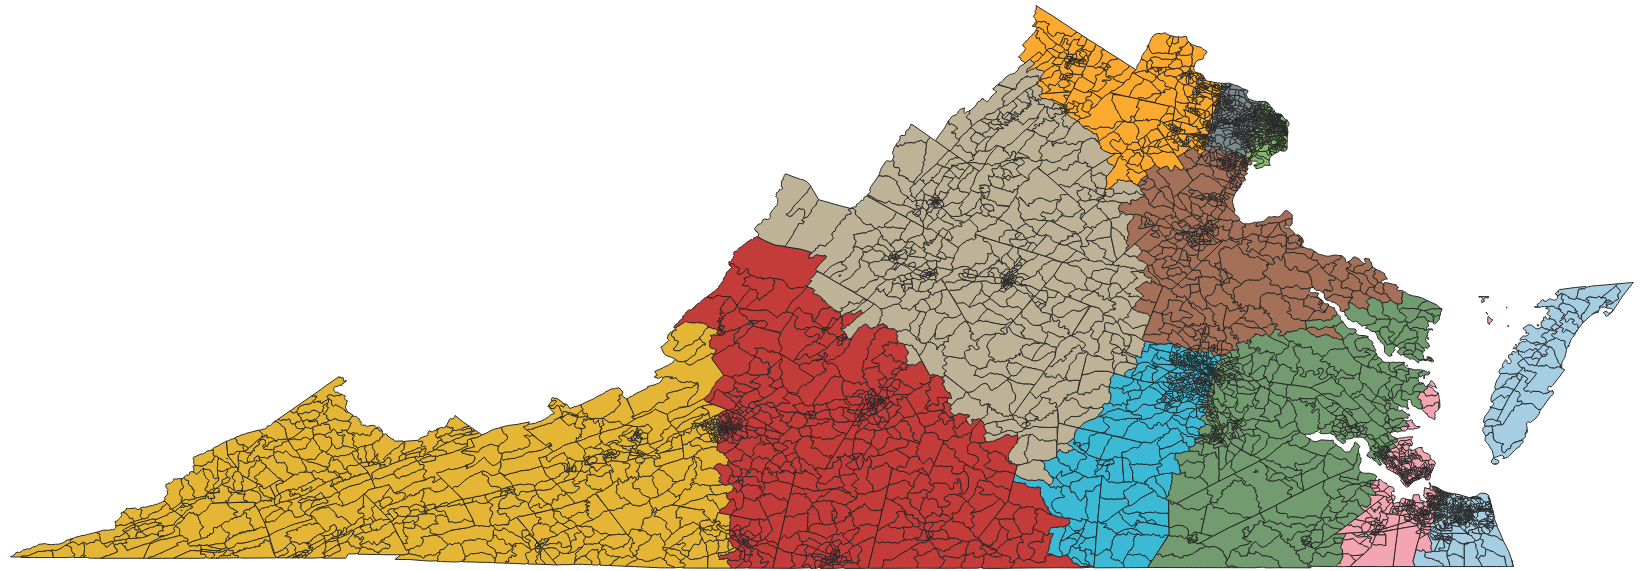
\includegraphics[width=.55\textwidth]{CBAssignments11}
	\caption{Census Block Assignments, before ``Dissolve" Operation}
	\label{fig:vmap11withcba}
\end{figure}

\begin{figure}[H]
	\centering
	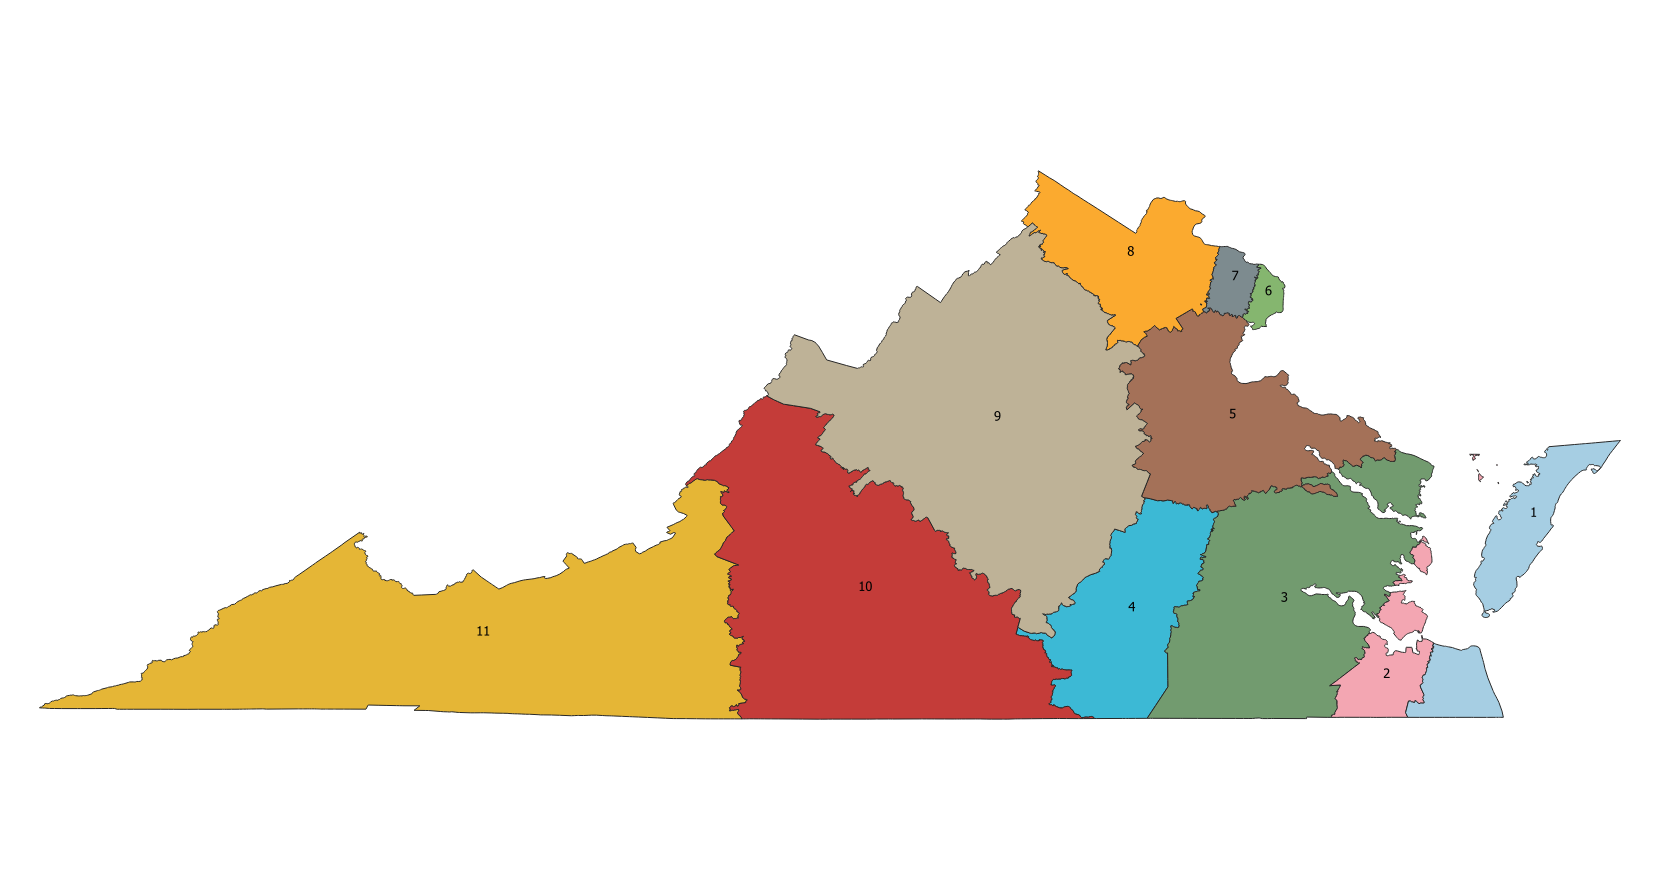
\includegraphics[width=.55\textwidth]{VA_Map_Whole_CB}
	\caption{Final Map that Respects Census Block Boundaries, with $k$ = 11}
	\label{fig:fmap11}
\end{figure}

\subsection{Metrics}

Now that we have created maps, we also want to generate metrics that will let us quantitatively compare maps. In general, the opposite of a gerrymandered map is a compact map, so these metrics will focus on determining how compact districts produced by a given method are.

\paragraph{Metric 1. Polsby-Popper Score}

The Polsby-Popper score for a district measure the ratio of area covered by a district, compared to the area of a circle with the same perimeter as the district\cite{OtherMetrics}. Obviously, for a circle, this ratio would be 1, but the score will become closer to 0 as the shape become more non-convex and disfigured. The formula is:
\begin{figure}[H]
	\centering
	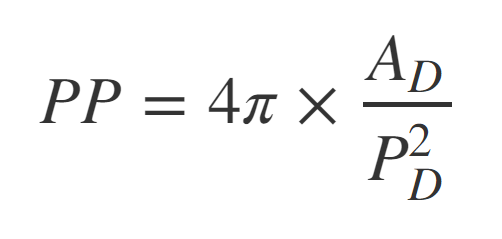
\includegraphics[width=.2\textwidth]{ppeq}
	\label{fig:ppeq}
\end{figure}

An example showing what the Polsby-Popper score represents is below:
\begin{figure}[H]
	\centering
	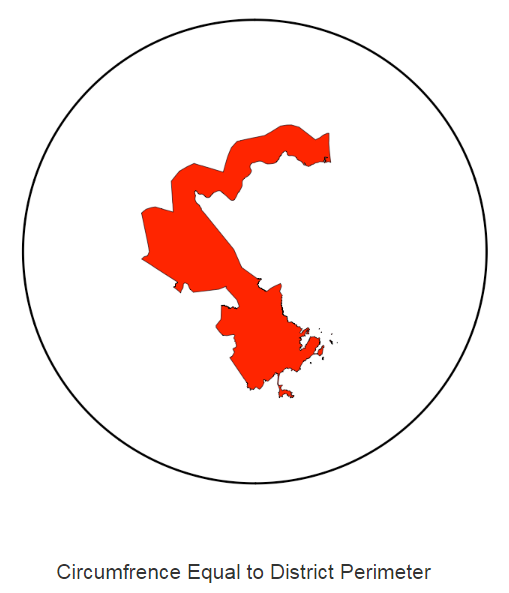
\includegraphics[width=.55\textwidth]{ppex}
	\caption{Polsby-Popper Score Example}
	\label{fig:ppex}
\end{figure}

For our project, this value was computed by the set of Python scripts ending with $Polsby\_Popper.py$. As expected, we utilize the Shapely library to compute the district area and perimeter values.

\paragraph{Metric 2. Convex Hull Ratio Score}

The next metric that we compute is the ratio between the area of the shape and the area of it's convex hull \cite{OtherMetrics}. One advantage of this computation is that it is not dependent on the perimeter of the shape, which may be large due to natural geography (rivers, shorelines, mountain ranges, \dots) that are largely beyond our control. The formula is:

\begin{figure}[H]
	\centering
	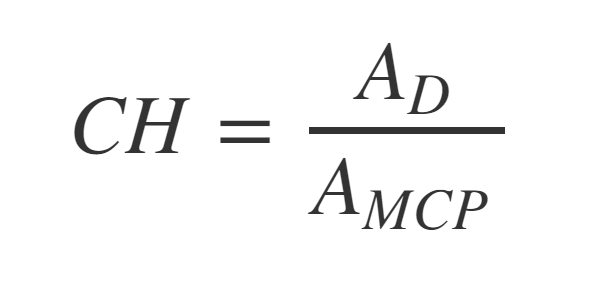
\includegraphics[width=.2\textwidth]{cheq}
	\label{fig:cheq}
\end{figure}

And an example, with the original Gerry-mander shape is:

\begin{figure}[H]
	\centering
	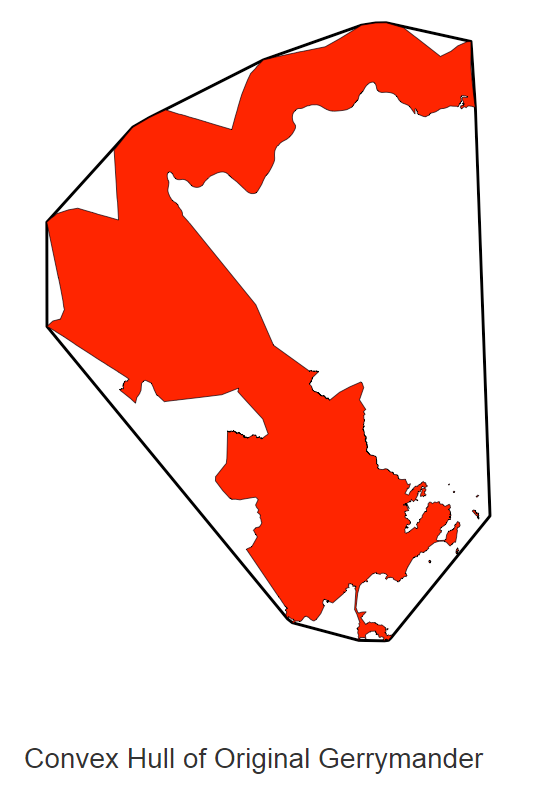
\includegraphics[width=.55\textwidth]{chex}
	\caption{Convex Hull Ratio Score Example}
	\label{fig:chex}
\end{figure}

In our code, these scores were computed by the $CH.py$ scripts, and again we use Shapely to find the district areas and the convex hull.

\paragraph{Metric 3. Average Distance to Centroid, based on Population}

For this metric, we compute the average distance between a resident and the center of their district. This is a useful metric because it is an informal, but relatable estimate of how compact the district is. The idea for this computation comes from Brian Olson, who used it to justify the compactness of many of the maps that he created. Note that this metric is influenced by the population distribution, so it matters where residents live within a district. The equation is:
\begin{figure}[H]
	\centering
	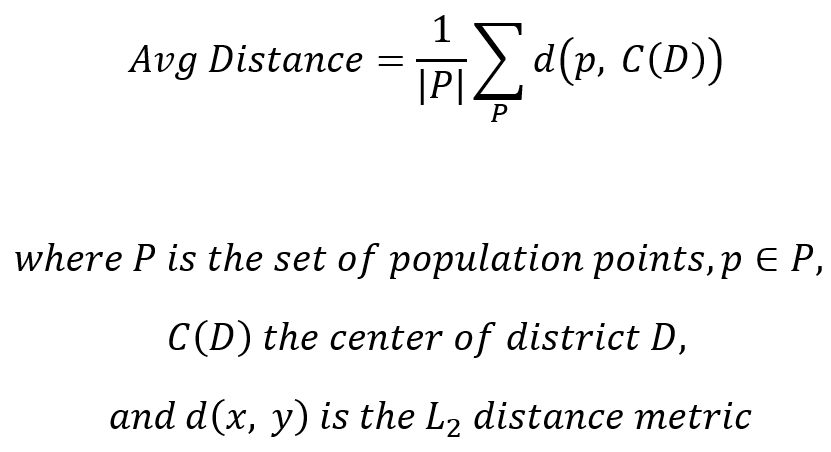
\includegraphics[width=.2\textwidth]{avgdisteq}
	\label{fig:avgdisteq}
\end{figure}

The values for this script were computed by the set of Python scripts named $Avg\_Dist.py$.

\paragraph{Metric 4. Average Distance to Centroid, based on Area}

The last metric that we consider is the average distance to the centroid, based exclusively on the geometry of the district shapes. To compute this we choose random sample points from the the districts and find the distance to the centroid. An exact geometric solution is possible, but the math is somewhat cumbersome, and this method gives results that are good enough.

\medskip

Note that our implementation uses the center of census blocks as the input points, and then weights each distance based on the area of the census block. Random sampling may be better, but there are typically several hundred census blocks per district, so the difference is negligible.

\medskip

Note that these values are computed in parallel with the previous metric in the same set of scripts.

\section{Results and Findings}

In this section we will present our final maps and the results or our metric computations. In addition, we will go into some discussion about the results.

\subsection{Final Map Comparison}

The following six maps are presented below.

\begin{enumerate}
	\item Current Virginia Congressional Districts
	\item Our Proposed Virginia Congressional Districts
	\item Current Virginia State Senate Districts
	\item Our Proposed Virginia State Senate Districts
	\item Current Virginia House of Delegates Districts
	\item Our Proposed House of Delegates Districts
\end{enumerate}

\begin{figure}[H]
	\centering
	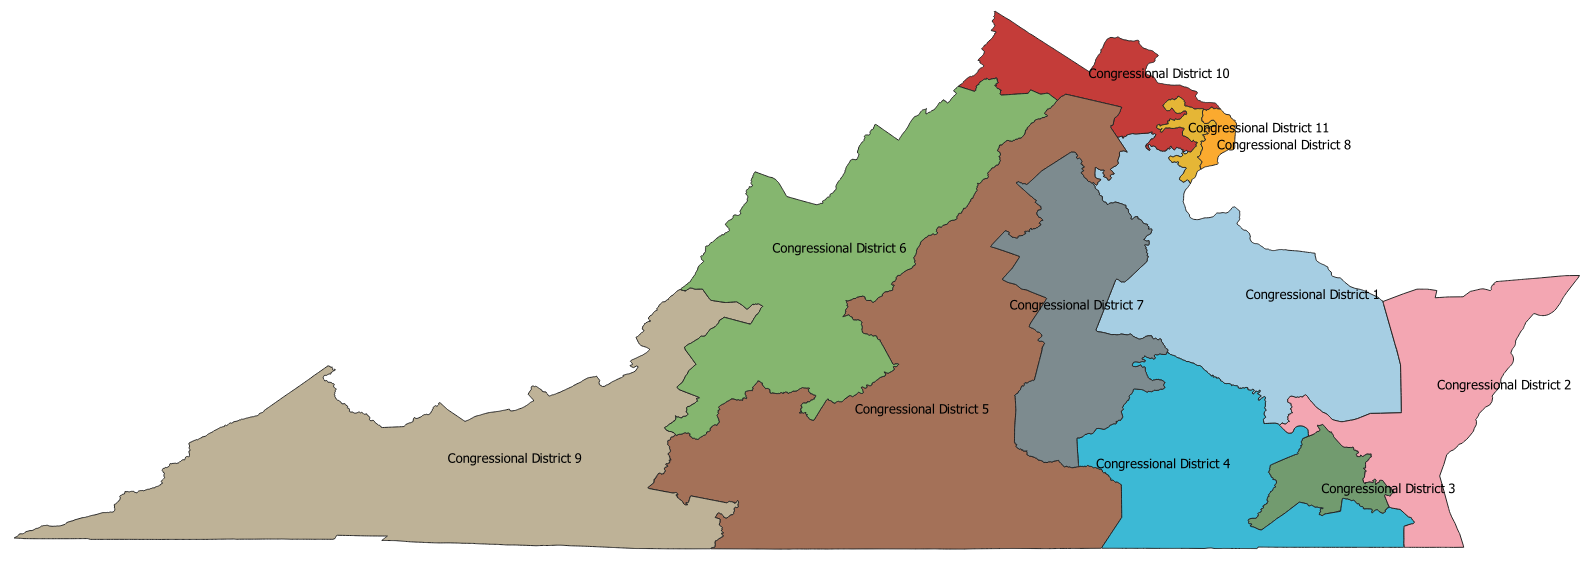
\includegraphics[width=\textwidth]{FinalMap1}
	\caption{Current Virginia Congressional Districts}
	\label{fig:fm1}
\end{figure}

\begin{figure}[H]
	\centering
	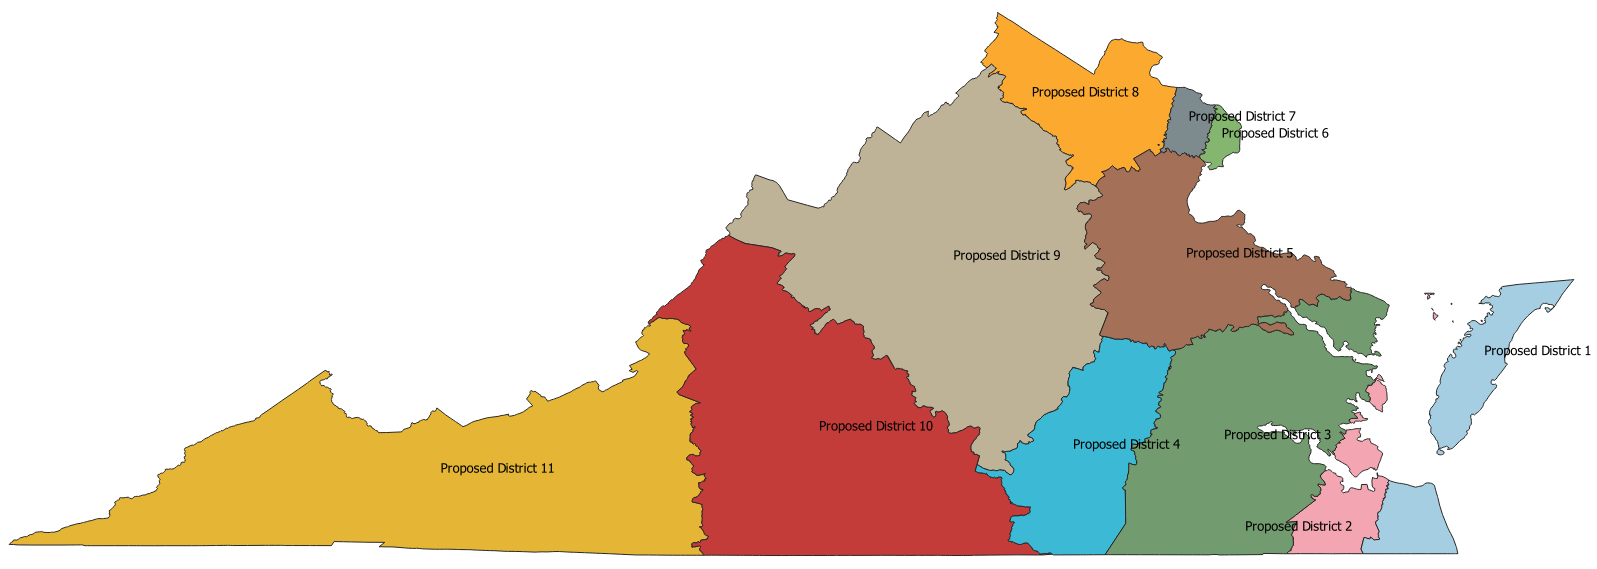
\includegraphics[width=\textwidth]{FinalMap2}
	\caption{Our Proposed Virginia Congressional Districts}
	\label{fig:fm2}
\end{figure}

\begin{figure}[H]
	\centering
	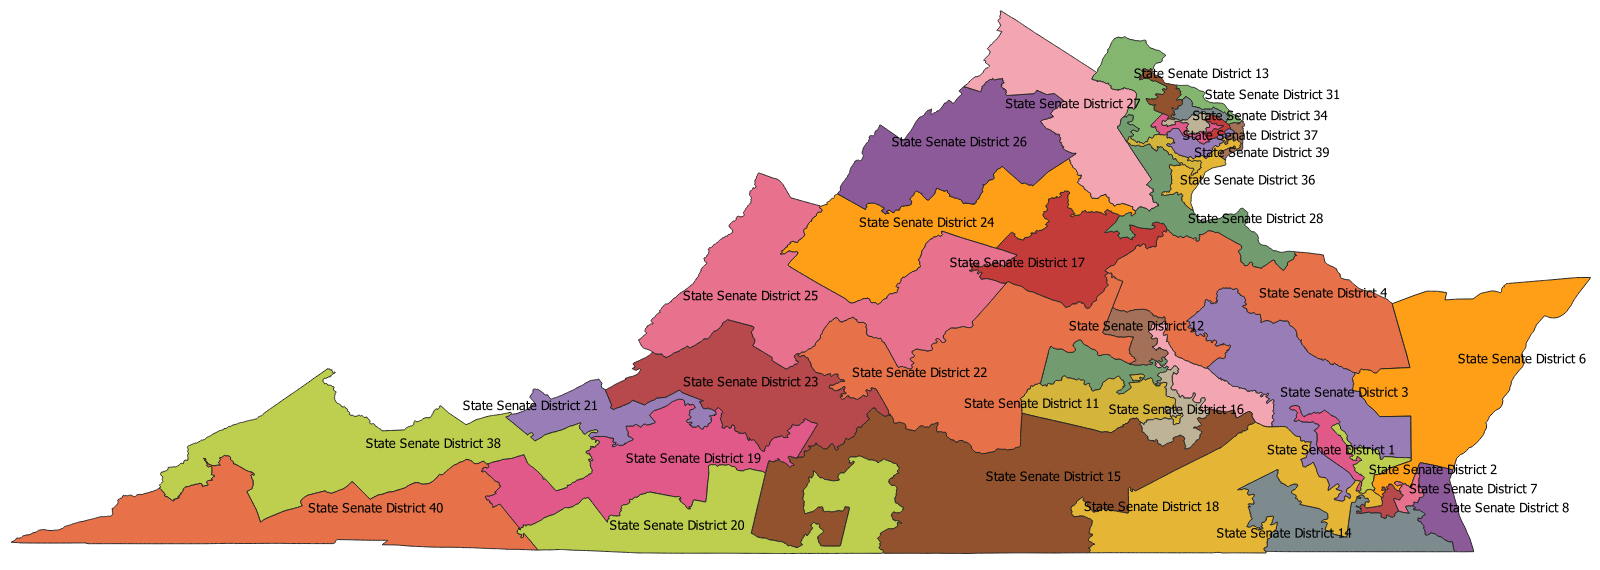
\includegraphics[width=\textwidth]{FinalMap3}
	\caption{Current Virginia State Senate Districts}
	\label{fig:fm3}
\end{figure}

\begin{figure}[H]
	\centering
	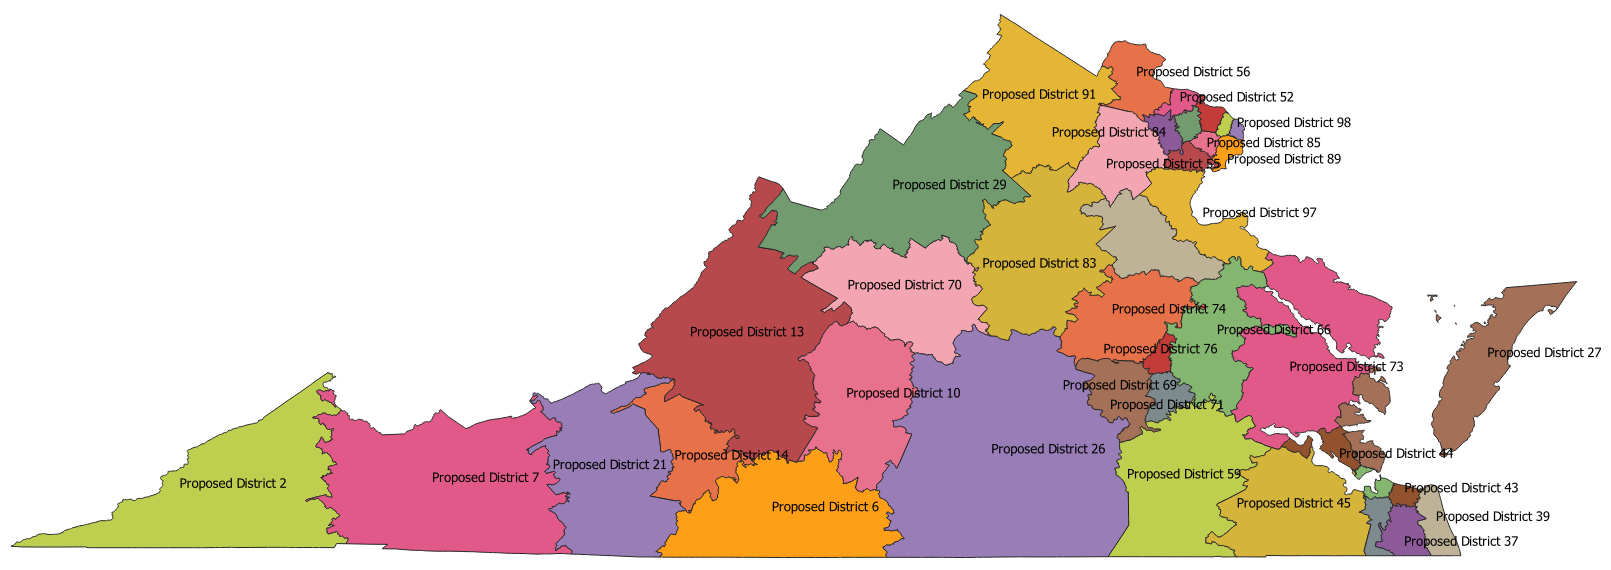
\includegraphics[width=\textwidth]{FinalMap4}
	\caption{Our Proposed Virginia State Senate Districts}
	\label{fig:fm4}
\end{figure}

\begin{figure}[H]
	\centering
	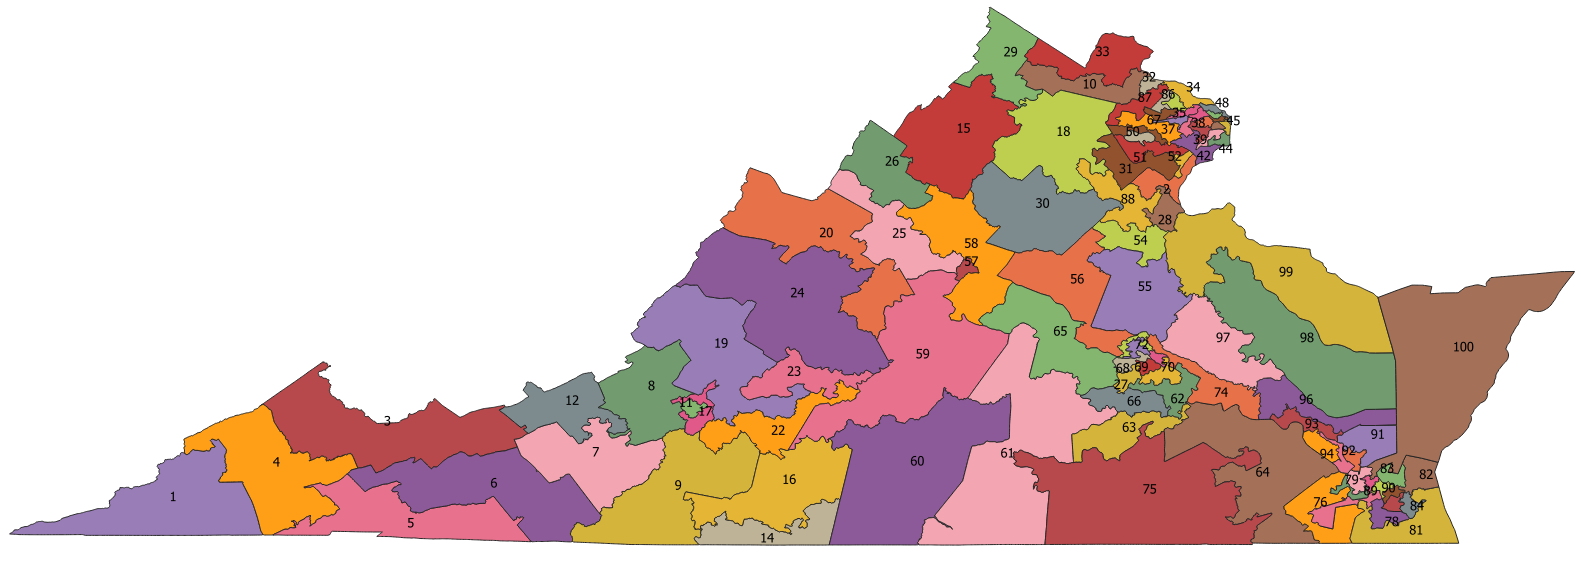
\includegraphics[width=\textwidth]{FinalMap5}
	\caption{Current Virginia House of Delegates Districts}
	\label{fig:fm5}
\end{figure}

\begin{figure}[H]
	\centering
	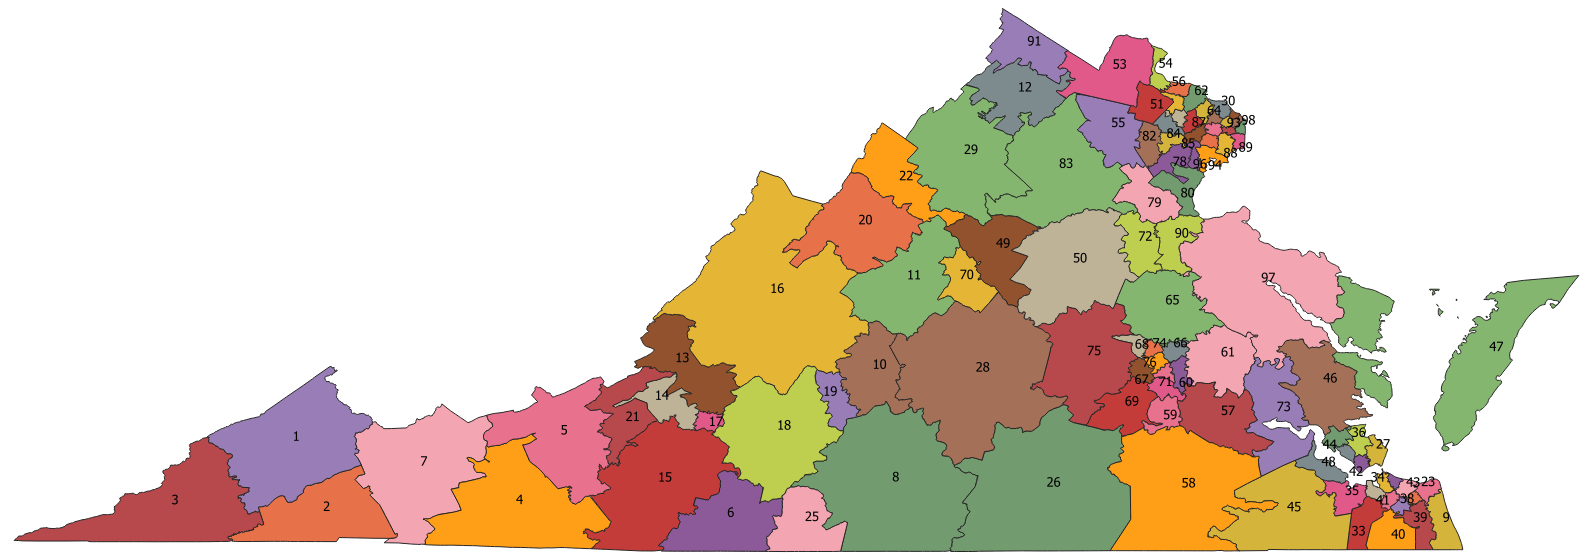
\includegraphics[width=\textwidth]{FinalMap6}
	\caption{Our Proposed House of Delegates Districts}
	\label{fig:fm6}
\end{figure}

\subsection{Metric Calculation Results}

In this section, we show the results for our four metrics that we described above. The computed values are shown here for the current 11 Virginia Congressional Districts, as well as the 11 proposed districts. In addition, we compute an average for each of the metrics, that can be used as a marker for the overall performance of each method.

\begin{figure}[H]
	\centering
	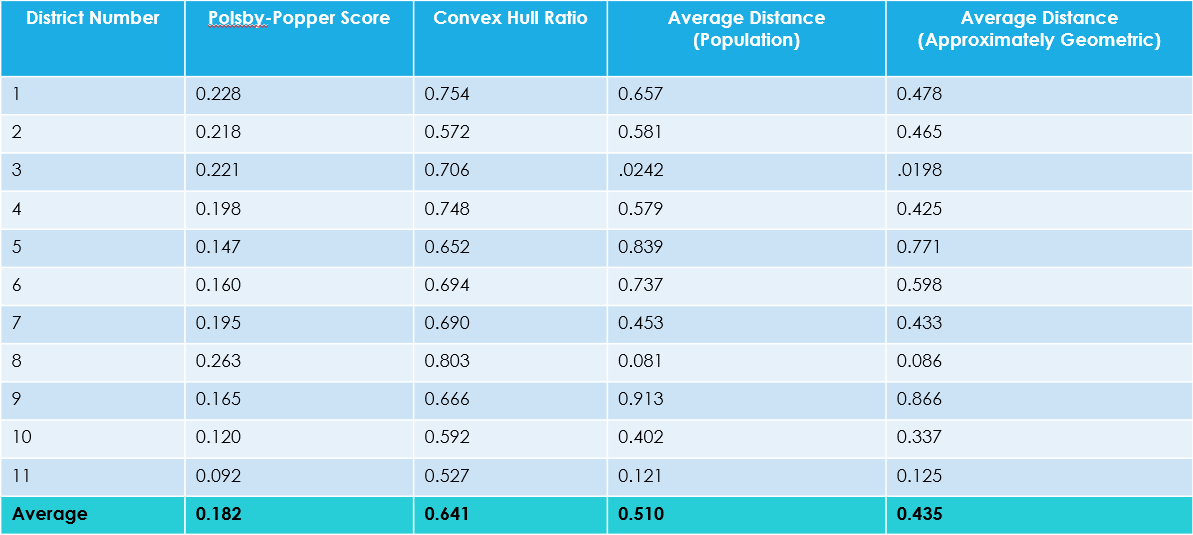
\includegraphics[width=\textwidth]{MetricsCurrent}
	\caption{Metrics for Current Congressional Districts}
	\label{fig:mc}
\end{figure}

\begin{figure}[H]
	\centering
	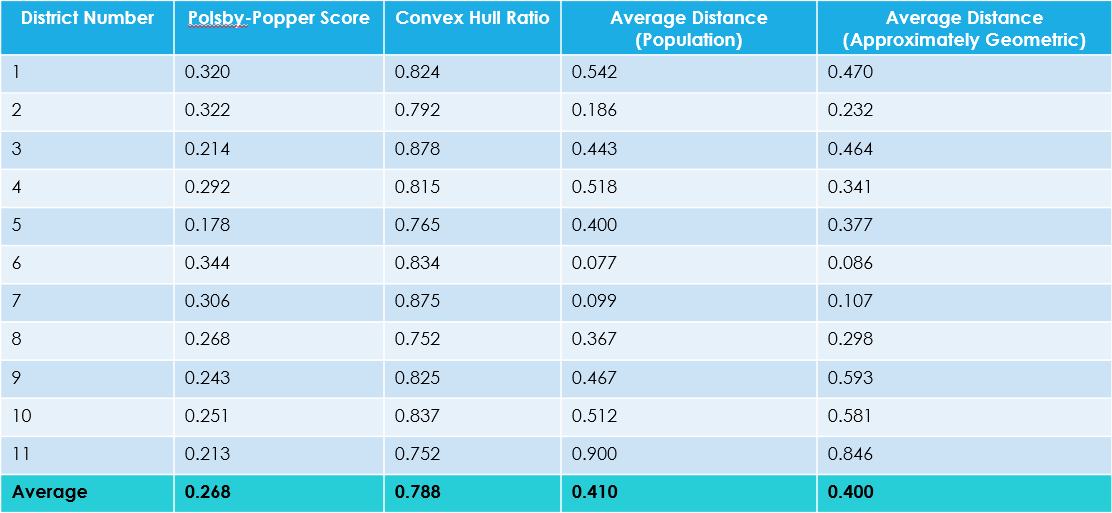
\includegraphics[width=\textwidth]{MetricsNew}
	\caption{Metrics for Proposed Congressional Districts}
	\label{fig:mn}
\end{figure}

As the figures show, the overall compactness is better with the new method. For both Polsby-Popper and Convex Hull, the average ratio using our method is higher, which indicates more compact districts. On the other hand, the average distance to center metrics are lower for our maps, which is again better because it means that we are dividing up the population more efficiently.

\medskip

Note that these metrics were presented in class as well, but they contained an error in the way that we were computing the average distances. This has been corrected, leading to the results above.

\subsection{Challenges and Lessons Learned}

As we mentioned in the previous section, one of the largest hurdles to overcome for this project was simply becoming familiar with how to work with geospatial information. There is a learning curve for understanding the shapefile data format, projections, new API's (Shapely and PyShp), and new UI functionality in QGIS. Researching information and finding data sources took more time than expected, with the retrieval of population data from the American Fact Finder website being particularly confusing.

\medskip

Another lesson learned was how important it is to keep data organized and adhere to particular conventions when generating and analyzing data. For example, organizing shapefiles, naming feature attributes consistently, and  generating reusable scripts is more difficult than I anticipated. In order to contunue this effort, I would need to reorganize my data files and document my processing pipeline.

\section{Conclusion and Future Work}

By generating new maps and computing metrics, this project demonstrated that we can indeed enact change that improves the gerrymandering situation we face. It is important to continue to make positive progress in this area so that states have real options available to them. In addition, continuing to raise public awareness is critical. In a few short months the 2020 Census will be taking place, with nationwide redistricting efforts occuring afterwards. A unified approach that combines the best features of structural reform for independent, bipartisan redistricting commissions and algorithmic techni	ques must be pursued to fight the issues we face.

\medskip

However, it is clear that there is plenty of work remaining to do that would further improve these results. A few examples are:
\begin{itemize}
	\item I demonstrated that it is possible to use the Voronoi cells from the balanced centroidal power diagram to generate a feasible map that does not break apart census blocks. However, there is no guarantee with this method that the equal population distribution across districts is maintained. More work would have to be done to determine the best way to iterate on the Voronoi output.
	\item Include more metrics and compute for additional maps, so that we have more data points to work with. In addition to compactness, we can also use historical data to find how competitive our proposed districts would be, for example. Ideally, we want a set of maps that are $representative$ of the entire population.
	\item Combine this method with other methods, such as the iterative techniques used by Brian Olson. Compare the maps generated by both methods and try to find a technique that incorporates the best features from both.
	\item Incorporate additional data, such as how important certain census boundaries are. For example, some boundaries coincide with county boundaries and might be better candidates to split districts on. In addition, we should prefer to utilize the census boundaries that are straight. Another example is that we should should prefer to use boundaries for larger roads and rivers that represent real division, rather than smaller streams and roads.
	\item We have shown that all of the individual steps in this process are efficient to be able to be performed at a state level in a few seconds. However, we need to find a way to combine steps, so that everything can be done programmatically, rather than relying on QGIS for key steps. Maintaining architectural flexibility during this process would be very important.
\end{itemize}

Lastly, this project was an excellent example of how concepts in Computational Geometry are applicable for real world problems. The operations needed to complete an undertaking such as this are driven by basic geometric algorithms that must scale to examples with thousands or millions of points that we encounter when working with state and national level data.

\bibliographystyle{plain}
\bibliography{William_Austin_Report}

\end{document}


